\chapter{System Design and Development}
\section{Introduction}
A remote monitoring system prototype has been developed (RDS) by combining mobile communication technologies and health care sensor networks. The system is built on top of open-source frameworks and its written in three different languages to meet all the requirements including Java, Python and C language. In this work, a minimum viable product has been developed to achieve the objective of this research. A first version of the prototype system is divided into four main parts:
\begin{itemize}
	\item{A health care device formed buy Arduino UNO board and a third party Health Version board shield. This device can accommodate different kind of health sensors that can collect different health vital signs. for the scope of this work the prototype only have three sensors including temperature sensor, SPO2 sensors and an Electrocardiogram (ECG) sensor}
	\item{An android smartphone device with a custom coded android application. This app is used to process the information from the health device and display the diagnosis content for the CHWs. A smartphone was chosen for this work since it has more addition free sensors. for instance, Global Positioning System (GPS), Camera and Mobile connections technology are used to collect more information about the patient and patient environment such as location information. the device also play an important role in delivering information to the remote Doctors for remote diagnosis and as well as to the CHWs}
	\item{A cloud application (Dashboard) is developed with a centralized database that stores information from the CHWs health devices. the dashboard categorizes the data and plot them to make them easy readable. It allows the Doctors to access the data and performs the diagnosis to generate final conclusions about the patient health status. Through this application Doctors can communicate directly to CHWs through their smartphones Through communication technologies that forms the forth path of the system}
	\item{
Finally, a communication part that is based on the google cloud messaging (GCM). this part allow the system to provide instant real time messages. Doctors can push messages without living the application environment, messages such as feedbacks, small intervention assistance and other to the mobile phones}
\end{itemize}

\section{System Architecture}

The figure below shows the system architectures including and the main building blocks of the system.
\begin{figure}[H]
\centering
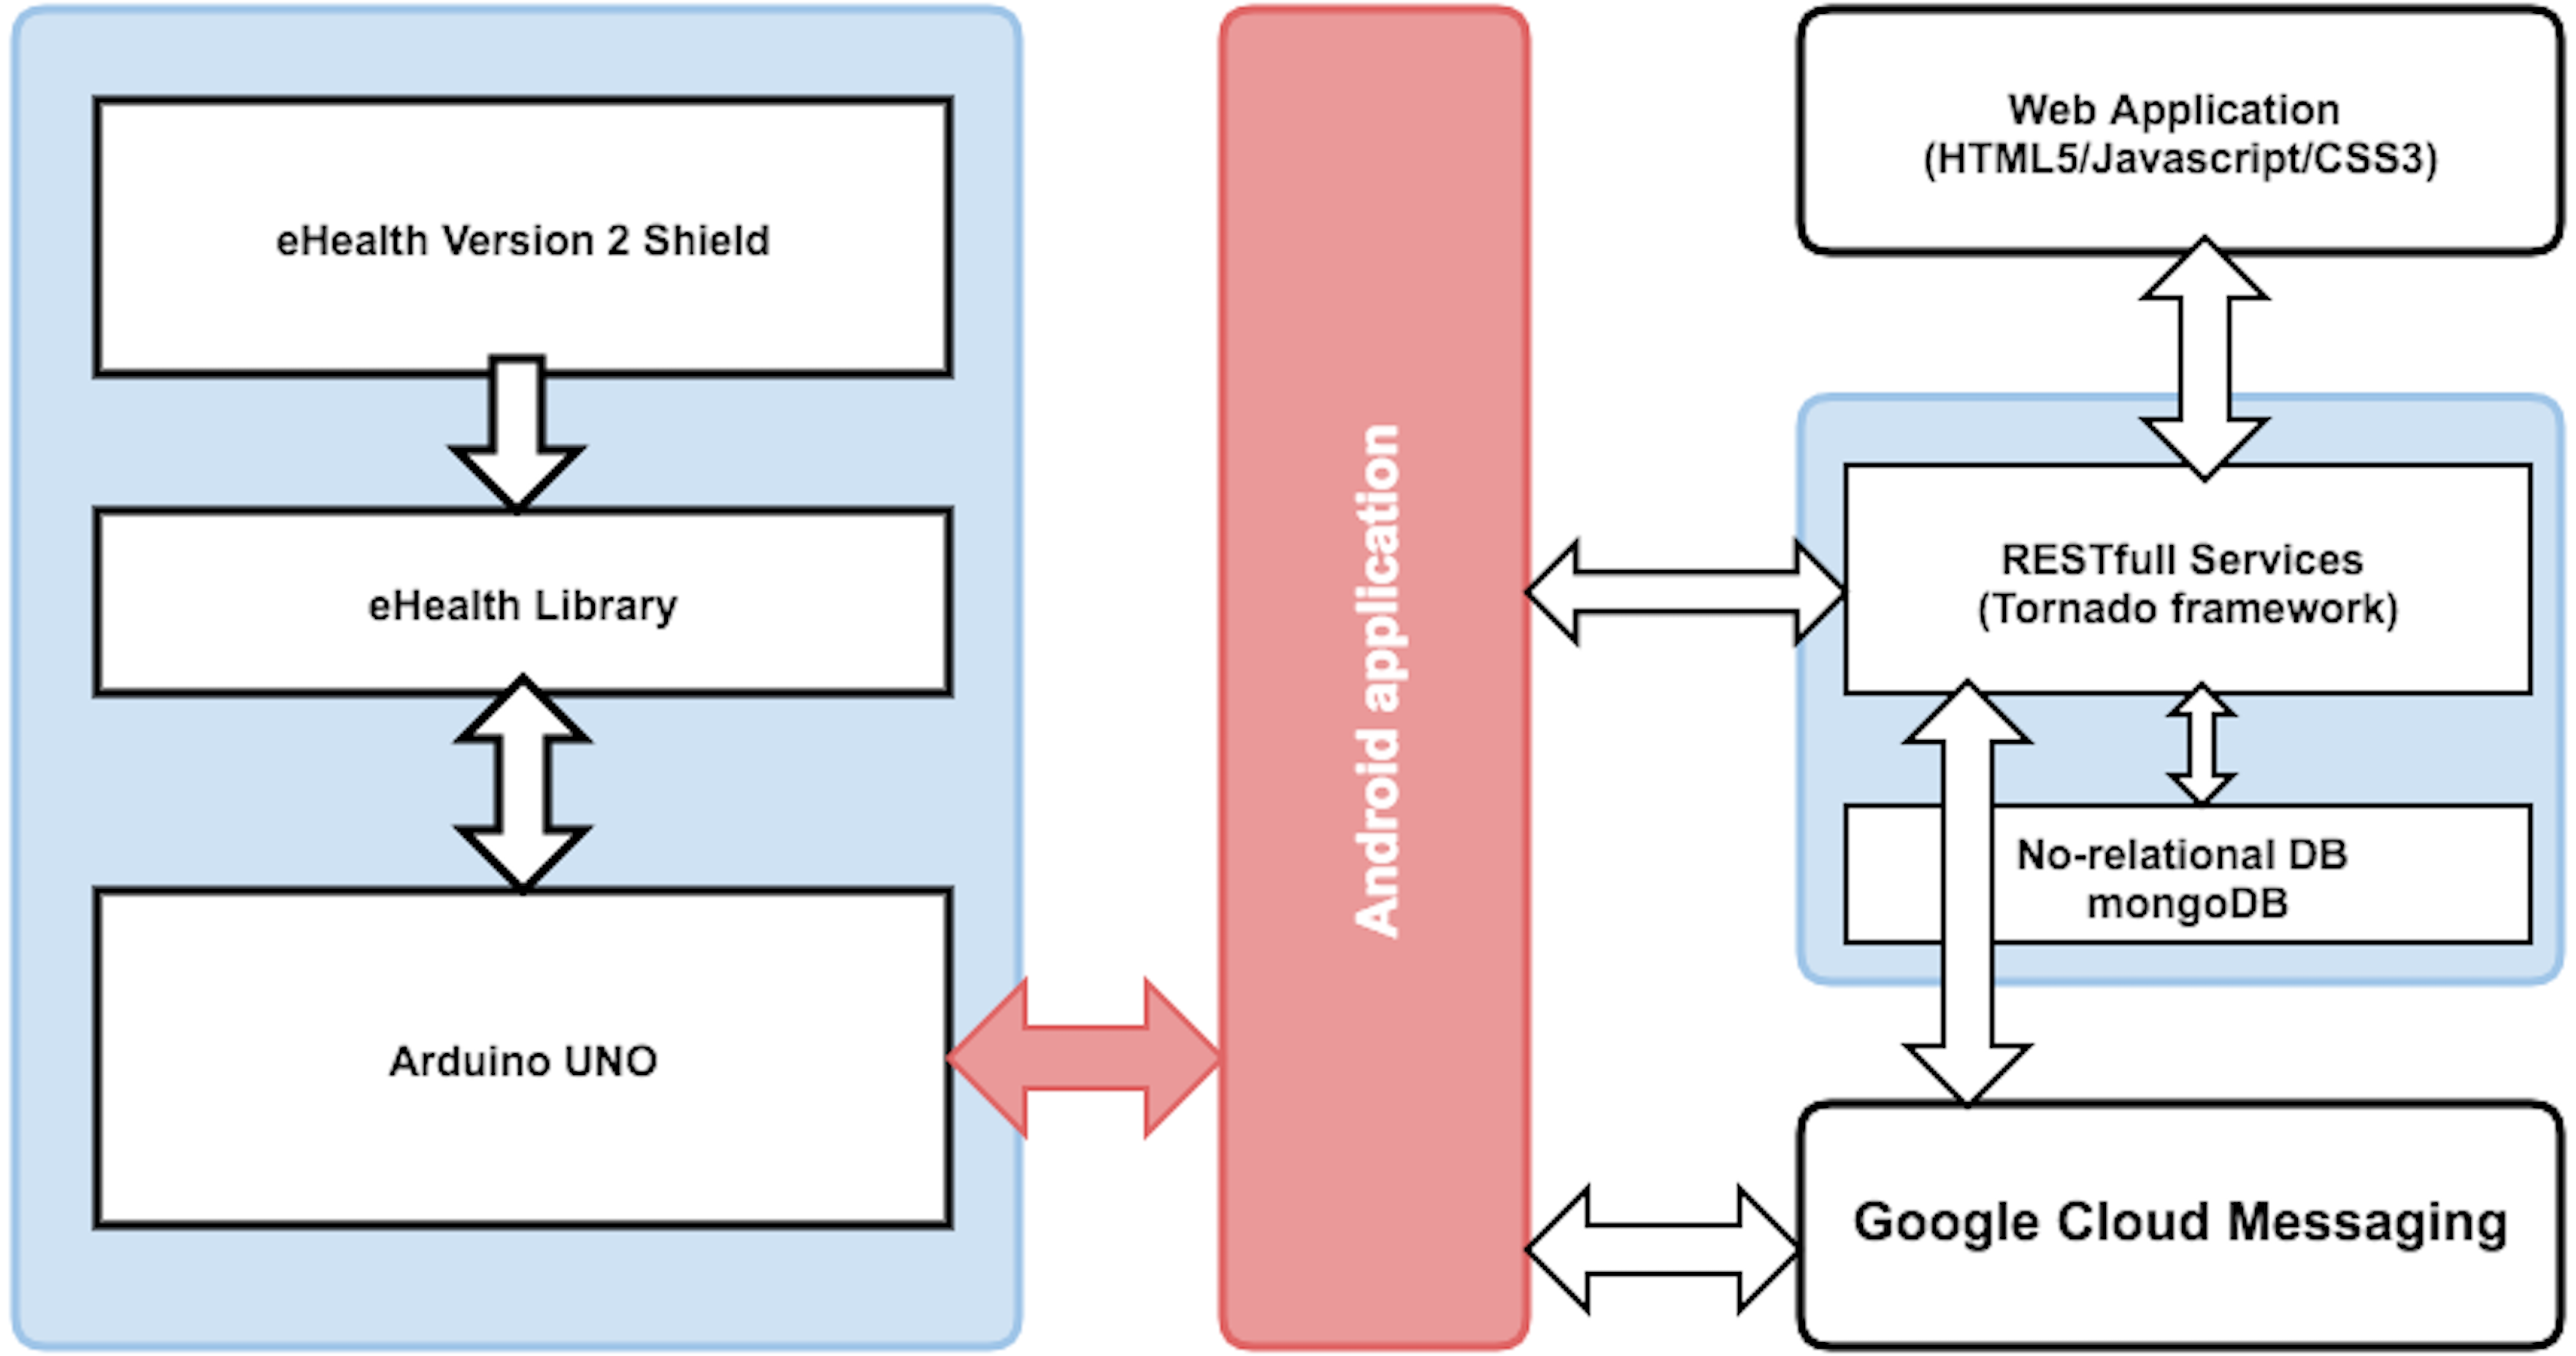
\includegraphics[width=15cm]{images/System_archutecture.png} % This scales the picture to
                                      % a width of 10cm
                                      % You can scale to the
                                      % width or height you need
%\end{center}
\caption{System Architecture}
\label{fig:fig-eg}
\end{figure}

In this work a portable health device is developed for HCWs that can plug into into mobile smartphone device. the concept as it shown in the system architecture figure above is to provide a full stack diagnosing tool based on mobile wireless communication by leveraging already existing technologies. The system is formed by four parts as it is mentioned above. (1) part one with is a health device with three different sensors and responsible of collecting different physiological data. this device consist of an Arduino UNO micro-controller that act as an interface between the device and the second part which is the Android device and application. the communication between the micro-controller and the android device is through USB with the use of build in Android USB HOST Libraries, (2) The android application act as an information display and relay to the third part of the system which act as the base station using mobile wireless technologies. (3) the web application consist of GUI, also this part is responsible of storing data, process and categorize them for better management, (4) the third part is linked to third party communication APIs that allows it to send back instant messages to the mobile device.

\section{Sensors}

As it is mentioned in the system architecture section, the system has three different sensors. Each sensor node measure different type of physiological information. In addition to this three sensors, the Android devices that is used to collect and display the data is also present with different sensors and some of which are used in this works to collect more information about the patients and there environment.
\begin{enumerate}
\item {\bfseries Temperature} Sensor: this sensor is used to measure patient body heat, this sensor can be place to the patient skin such as on the finger or on the leg
\item {\bfseries SPO2 (Peripheral Capillary oxygen saturation ) } sensor: this sensor is responsible of estimating the percentage number of oxygenated hemoglobin compared to the total amount of hemoglobin in the blood
\item {\bfseries ECG (Electro-Cardiogram )} sensor: this sensor is comprised with three electrodes positive, negative and neutral electrodes, that are placed on the patient skin. this sensor is responsible of measuring the electric activities of the patient heart for a certain amount of time
\end{enumerate}

The Sensor devices mentioned above are responsible of monitoring different physiological data of the patient. The table bellow show the specifications of various physiological data that are measured by the sensors.
\begin{table}[H]
\begin{center}
    \begin{tabular}{ |l|l|l| }
\hline
{\bfseries Parameters} & {\bfseries Specifications} \\ \hline
\multirow{5}{*}{Body Temperature} 
  & Hypotermia:  \textless $35$\textdegree C\\
  & Normal      : $36.5$\textdegree C to $37.5$\textdegree C \\
  & Hyperthermia/ Fever: \textgreater $37.5$\textdegree C to $38.3$\textdegree C\\
  & Hyper pyrexia: \textgreater $40.0$\textdegree C to $41.5$ \textdegree C \\ \hline
Oxygen saturation in blood (SaO2) & 0\% to 100\% \\ \hline
\multirow{2}{*}{Electrocardiogram (ECG)} 
 & Frequency: 0.5Hz – 100 Hz  \\
 & Amplitude: 0.25 – 1mV\\
\hline
\end{tabular}
\end{center}
\caption{Various vital parameters measured by the sensors}\label{vital}
\end{table}

\section{Design and Implementation process}


\section{System Requirements}

The designed system is highly described in the above sections of the chapter 4. in this section will try to describe basic requirements for each component of the system to allow the fulfillment of required use case scenarios.

n addition, the system was build around open-source frameworks and eHealth version two kit that was selected to experiment and test out our hypothesis.

\begin{itemize}
\item To allow the CHWs have the tools, in this case sensors and have the applied to patients.
Requirements:
	\begin{enumerate}
		\item eHealth version two kit, This kit must allow all the selected sensors and collect all signals from them
		\item Arduino Uno micro controller, The Arduino should have all the logic and functionality to process the data
		\item eHealth Library software, this library is integrated to allow the eHealth kit to work with Arduino micro controller, in addition this library should facilitate the customization and calibration of sensors
	\end{enumerate}
\item The system should allow the CHWs to visualized the data collect from the sensors and act accordingly. For better decision making the system should also have the capability of sending the data to remote Doctors for further analysis and generate feedbacks to assist CHWs. Requirements:
	\begin{enumerate}
		\item A smart phone device that runs android version 4.0.3 (Ice Cream Sandwich) and higher is required
		\item To connect the Arduino Uno to the smart phone An OTG cable is required for transferring the data from the micro   controller to the smartphone. In addition, this cable will allow the smart phone to power up the micro controller
		\item Google Cloud Messaging (GCM) libraries and configurations, to allow the smart phone to generate alert and notification for The CHWs
	\end{enumerate}
\item A cloud based application (Server Application) should be implemented to store and analyze data for the Doctors to judge and make some form of conclusions. Requirements:
	\begin{enumerate}
		\item RESTFull server with minimum data manipulation web services with some business logic
		\item no-relation database system ( Mongoldb Database) to store the big data generated by the sensors and integrate different resources from different third party APIs
	\end{enumerate}
\end{itemize}

The above requirements are designed to develop a minimum viable product functionality of the prototype. They are also designed to achieve the goal of building a cost effective system that can allow the HCWs to detect and prevent illness at their early stage. Hardware and software details will be discussed in the following points according to the requirements specified in this section. 

\section{System hardware}
\subsection{eHealth version two kit Shield Board}

The eHealth sensor shield platform was developed to be used in the health care sector. the board can be interfaced with different other micro controllers such as Arduino, and a full stack mini computer such as Raspberry Pi. The board was build by cooking hack and can support 10 different health care sensors: body temperature, pulse and Oxygen saturation in blood (SPO2), electrocardiogram (ECG), Airflow sensor, glucometor, galvanic skin response, blood pressure sensor, accelerometer (Patient position) and electromyograph sensor(EMG).
\begin{figure}[H]
\centering
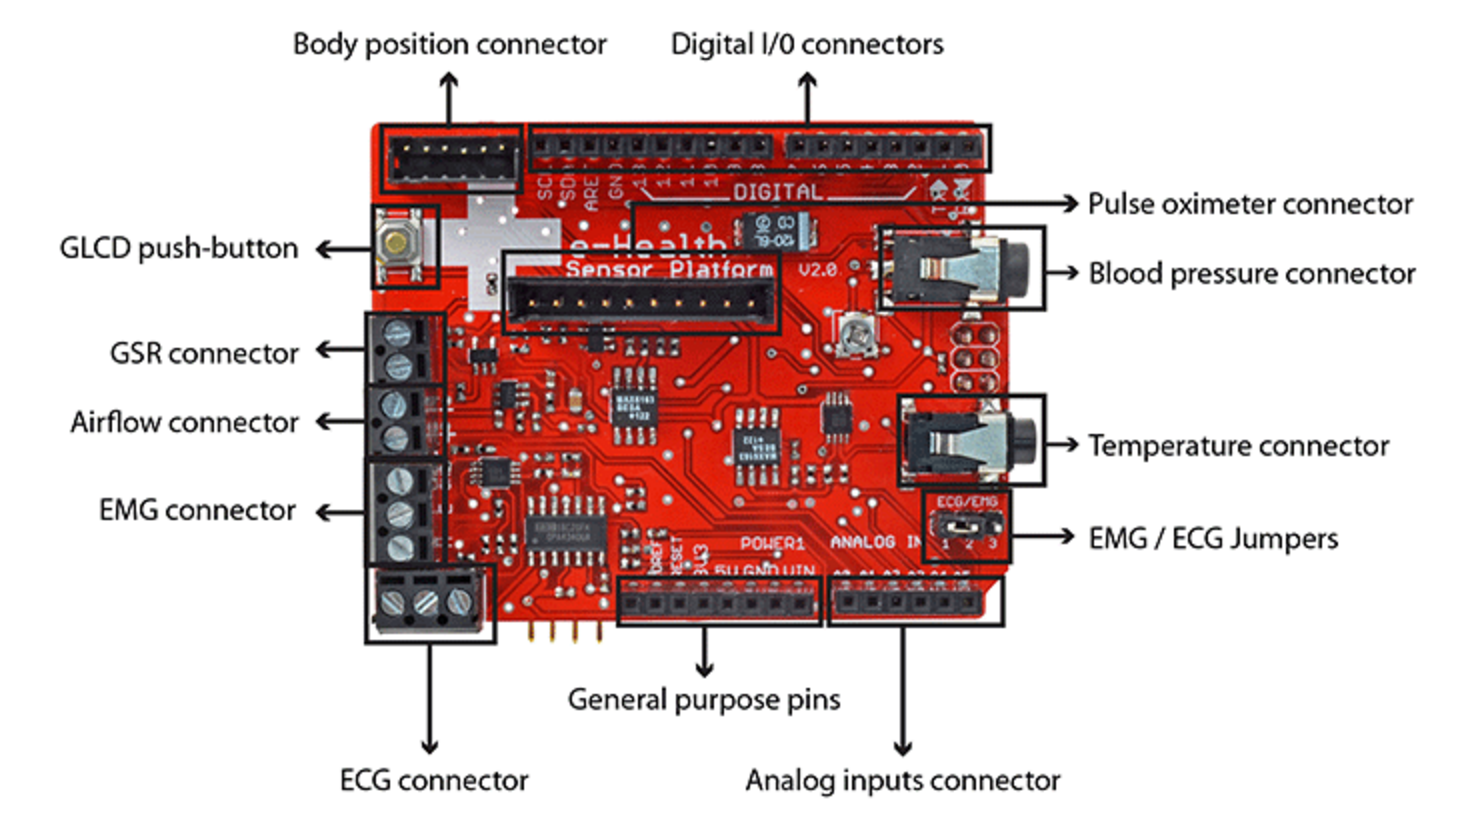
\includegraphics[width=15cm]{images/ehealth_kit.png} % This scales the picture to
                                      % a width of 10cm
                                      % You can scale to the
                                      % width or height you need
%\end{center}
\caption{eHealth sensor shield platform}
\label{fig:fig-eg}
\end{figure}

The board is also capable of supporting a number of communication protocols such as wifi and bluetooth shield board to exchange data with other devices or cloud applications. in this work only three sensors body temperature, ECG and SPO2 sensors were selected to conduct the experiments and implement the prototype.

\subsection{Arduino UNO}

The RDS health device is based on Arduino microprocessor technology. The Arduino is the core part since it is used to collect and process the data from the sensors through the health sensor shield board.

\begin{figure}[H]
\centering
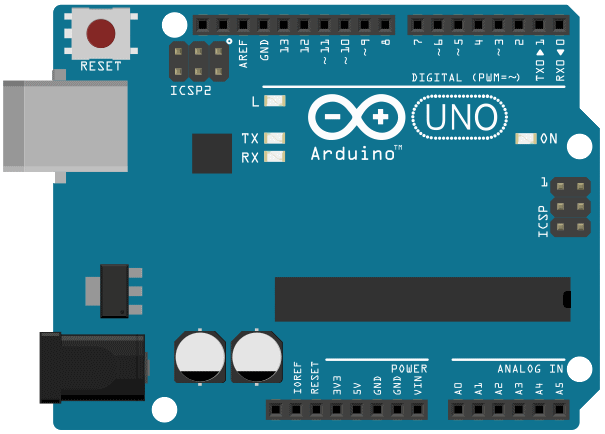
\includegraphics[width=8cm]{images/arduino-uno.png} % This scales the picture to
                                      % a width of 10cm
                                      % You can scale to the
                                      % width or height you need
%\end{center}
\caption{Arduino UNO micro controller board}
\label{fig:fig-eg}
\end{figure}

The figure two above show the Arduino board used in the system. It provides the environment that is easy accessible and compatible to the Android environment. The eHealth shield sensor board shield was build on to work with Arduino board and its health library is easily integrated in the Arduino development environment (IDE). The figure bellow shows the Arduino Uno specification requirements used in the system.

\begin{table}[H]
\begin{center}
    \begin{tabular}{ |l|l|l| }
\hline
{\bfseries Parameters} & {\bfseries Specifications} \\ \hline
Microcontroller & ATmega328P \\ \hline
Operating Voltage & 5V \\ \hline
Input Voltage (recommended) & 7-12V \\ \hline
nput Voltage (limit) & 6-20V \\ \hline
Digital I/O Pins & 14 (of which 6 provide PWM output) \\ \hline
PWM Digital I/O Pins & 6 \\ \hline
Analog Input Pins & 6 \\ \hline
DC Current per I/O Pin & 20 mA \\ \hline
DC Current for 3.3V Pin & 50 mA \\ \hline
\multirow{2}{*}{Flash Memory} 
 & 32 KB (ATmega328P)  \\
 & of which 0.5 KB used by bootloader\\
\hline
SRAM & 2 KB (ATmega328P)\\ \hline
EEPROM & 1 KB (ATmega328P) \\ \hline
Clock Speed & 16 MHz \\ \hline
Lenght & 68.6 mm \\ \hline
Width & 53.4 mm \\ \hline
Weight & 25 g \\ 
\hline

\end{tabular}
\end{center}
\caption{Arduino Microcontroller Technical specification\cite{ArduinoUnoSpecs}}\label{Microcontroller}
\end{table}


\subsection{USB OTG cable }
USB OTG cable is a special USB cable using standards that can allow an android smart phone connect and communicate with peripheral devices. USB OTG (USB On The Go) was developed to give a mobile phone the power to enable other devices, by enabling USB host feature on the android phone. A smart phone with a USB host enabled acts a hub to all connected devices and can be used to addition devices such as keyboards and other devices.

USB OTG cable was used in this work to enable the smart phone as the gateway and can read and process the information from the sensors through the micro controller.

\subsection{Android smart phone}

The android smartphone (Samsung Galaxy S4) unit is used to read data from the health sensors using OTG cable as an interface. By using the smartphone processing power the custom made application processes the data and visualize them on the screen for further decision making on the ground by CHWs. In addition, the addition smartphone sensors are used to collect more information such as GPS and camera. Also it can temporarily store data locally in a SQLite database as a transitional database before sending data to the cloud for avoiding loss of data in case there is a network problem. The OTG cable was chosen not only to transfer data back and forth between the android smartphone and the e-health device but also to pawer the e-health device with the smartphone battery. the following table show the specification of the smart phone used in this study.

\begin{table}[H]
\begin{center}
    \begin{tabular}{ |l|l|l| }
\hline
{\bfseries Parameters} & {\bfseries Specifications} \\ \hline
Screen size & 5.1 in \\ \hline
\multirow{2}{*}{\bfseries Storage} 
 & 16/32 GB internal,  \\
 & MicroSD slot up to 128 GB\\
\hline
\bfseries Operating System & Androind Kit Kat\\ \hline
\multirow{2}{*}{\bfseries Battery Life} 
 & Up to 21 hours talk,  \\
 & up to 67 hours music\\
\hline
\multirow{2}{*}{\bfseries Camera} 
 & 16 MP primary,  \\
 & 2 MP fron-facing\\
\hline
\multirow{2}{*}{\bfseries Processor} 
 & Qualcomm MSM8974AC,  \\
 & Snapdragon 801, Quad-core 2.5GHz krait 400\\
\hline
\end{tabular}
\end{center}
\caption{Android smartphone technical specification}\label{Smart phone}
\end{table}

\subsection{Server hardware}

The server computer will be used to host the web application and store the data from the mobile smartphone. The server computer hardware will be able to handle all the request form the authorized users and have the power to perform or complex data manipulation. the following table show the minimum requirements of a ubuntu server.

\begin{table}[H]
\begin{center}
   \begin{tabular}{|l|l|l|l|l|}
    \hline
    \bfseries Install Type & \bfseries RAM & \bfseries CPU & \multicolumn{2}{ l| }{\bfseries Hard drive space} \\
   \cline{1-5}
   & & & \bfseries Base system & \bfseries All tasks Installed \\ 
\hline
   \bfseries Server(Standard) & 1 gigahertz & 512 megabytes & 1 gigabytes & 1.75 gigabytes \\
\hline
   \bfseries Server(Minimum) & 300 megahertz & 192 megabytes & 700 megabytes & 1.4 gigabytes \\
\hline
  \end{tabular}
\end{center}
\caption{Recommanded minimun Lunix server requirement}\label{Server}
\end{table}

In this study a ubuntu server was used with ubuntu version 14.0.0 . for storing the data a non-relational database Mongodb was configured to save the data as collections in a non-relation fashion. The server is also configured to host a python server application with several other python package for data visualization and analysis.

\section{System Software Design and Tools}

In this section Software design and components are discussed in more details. Tools as well as libraries used in different levels of the system will be also discusses with the functionalities they implements. Sample codes to show some of the functionalities may or may not be shown here to be found in the code snippet on appendix pages.

\subsection{e-Health device}

The device is build on top of the e-health board kit that was developed by cooking hack, and it comes with a number of sensors. The kit is bundled with a library that provide build-in methods functions to collect and gather data from the different sensor node. The diagram below illustrates the software building block and the information flow mechanisms of the designed device. The device is compatible with Arduino micro-controller and Raspberry pi. In this study we chose to work with Arduino in this study for its many advantage it brings such as interfacing with a smart-phone easily and also provides an easy to use programming environment.


\begin{figure}[H]
\centering
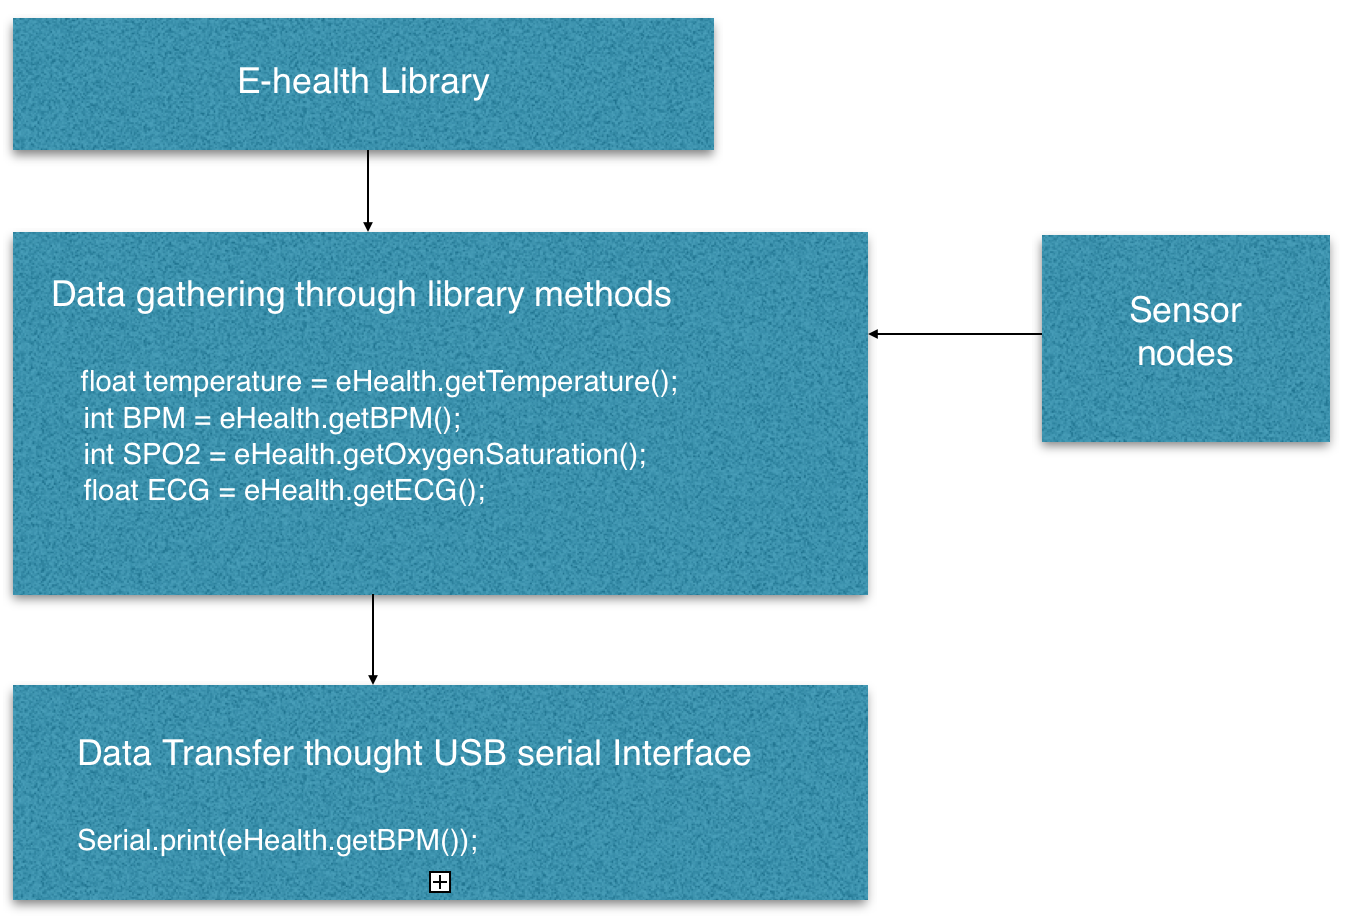
\includegraphics[width=13cm]{images/ehealth_devices_design.png} % This scales the picture to
                                      % a width of 10cm
                                      % You can scale to the
                                      % width or height you need
%\end{center}
\caption{eHealth device building blocls and algorithm design}
\label{fig:fig-eg}
\end{figure}


Arduino IDE is used to write functionalities that allow to access to sensors and collect sensor readings through the eHealth library that is written in C++. The IDE is also used to alter the library code to enhance the sensors readings. More libraries where used such as serial-communication library for the Arduino to communicate with the mobile handset via bluetooth communication protocol for further experiments.


\subsection{Android Application}


Android Studio IDE was used to write the android application that reads data from the Arduino micro controller via the OTG cable in the form of bytes. Android Application is written using Java for android and uses a number of open-source such as the google play services library for notification often called Google Cloud Messaging Library and the OKHttp android library for data transmission over the internet to the cloud application. With the use of OKHttp android library the android smart-phone does not only used to read information, process them and to store them temporary but also as a hub between the sensor devices and the cloud application. The diagram bellow show the class design diagram of the android application. The diagram show all the minimum viable functionality of the prototype and all third party services to enhance its usability.


\begin{figure}[H]
\centering
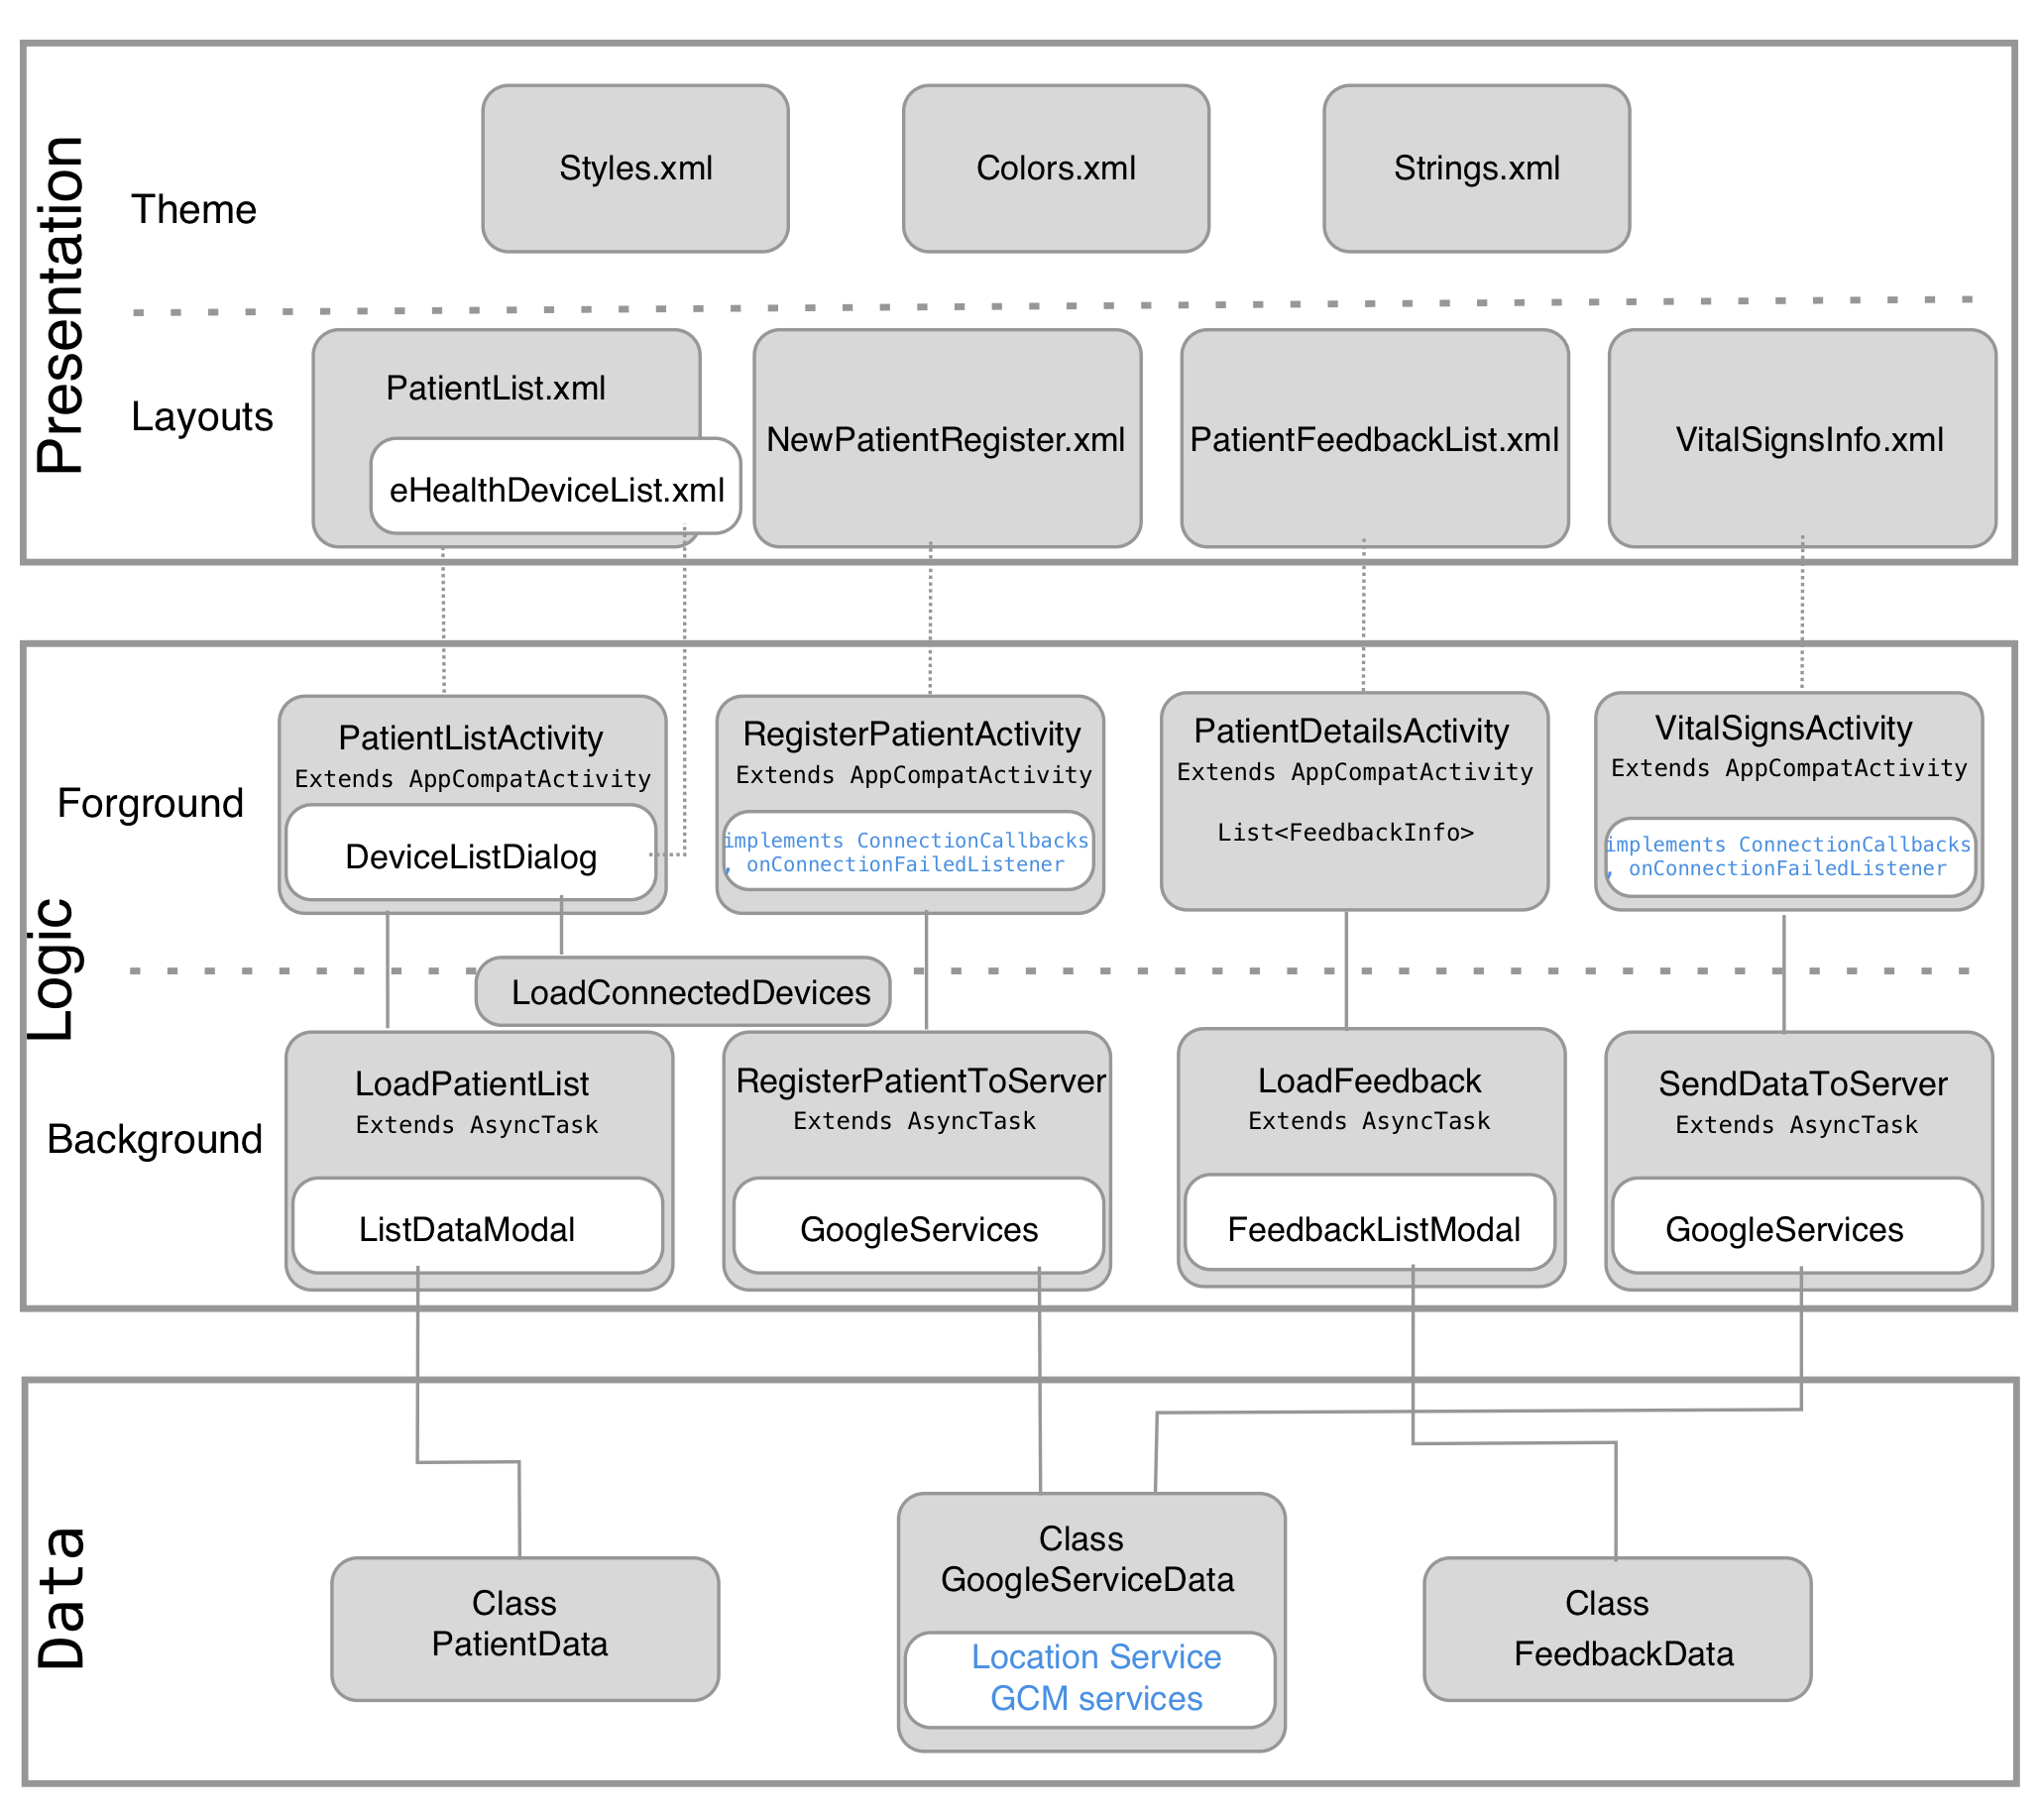
\includegraphics[width=13cm]{images/android_application_design.png} % This scales the picture to
                                      % a width of 10cm
                                      % You can scale to the
                                      % width or height you need
%\end{center}
\caption{Android Application software design classes}
\label{fig:fig-eg}
\end{figure}


\subsection{Server Application}


the server application is responsible of providing more capability of processing and storing data in a more fashioned way. As described in the previous chapters the cloud application uses web technologies and this allows the dashboard application to be accessed easily on different devices that are connected to the internet. Allowed medical Doctors and Nurses can access information at any time and provide the assistance to CHWs through the same cloud application. The following diagram show the major components of the cloud applications and the processes involved in charing data with the Android mobile application.
\begin{figure}[H]
\centering
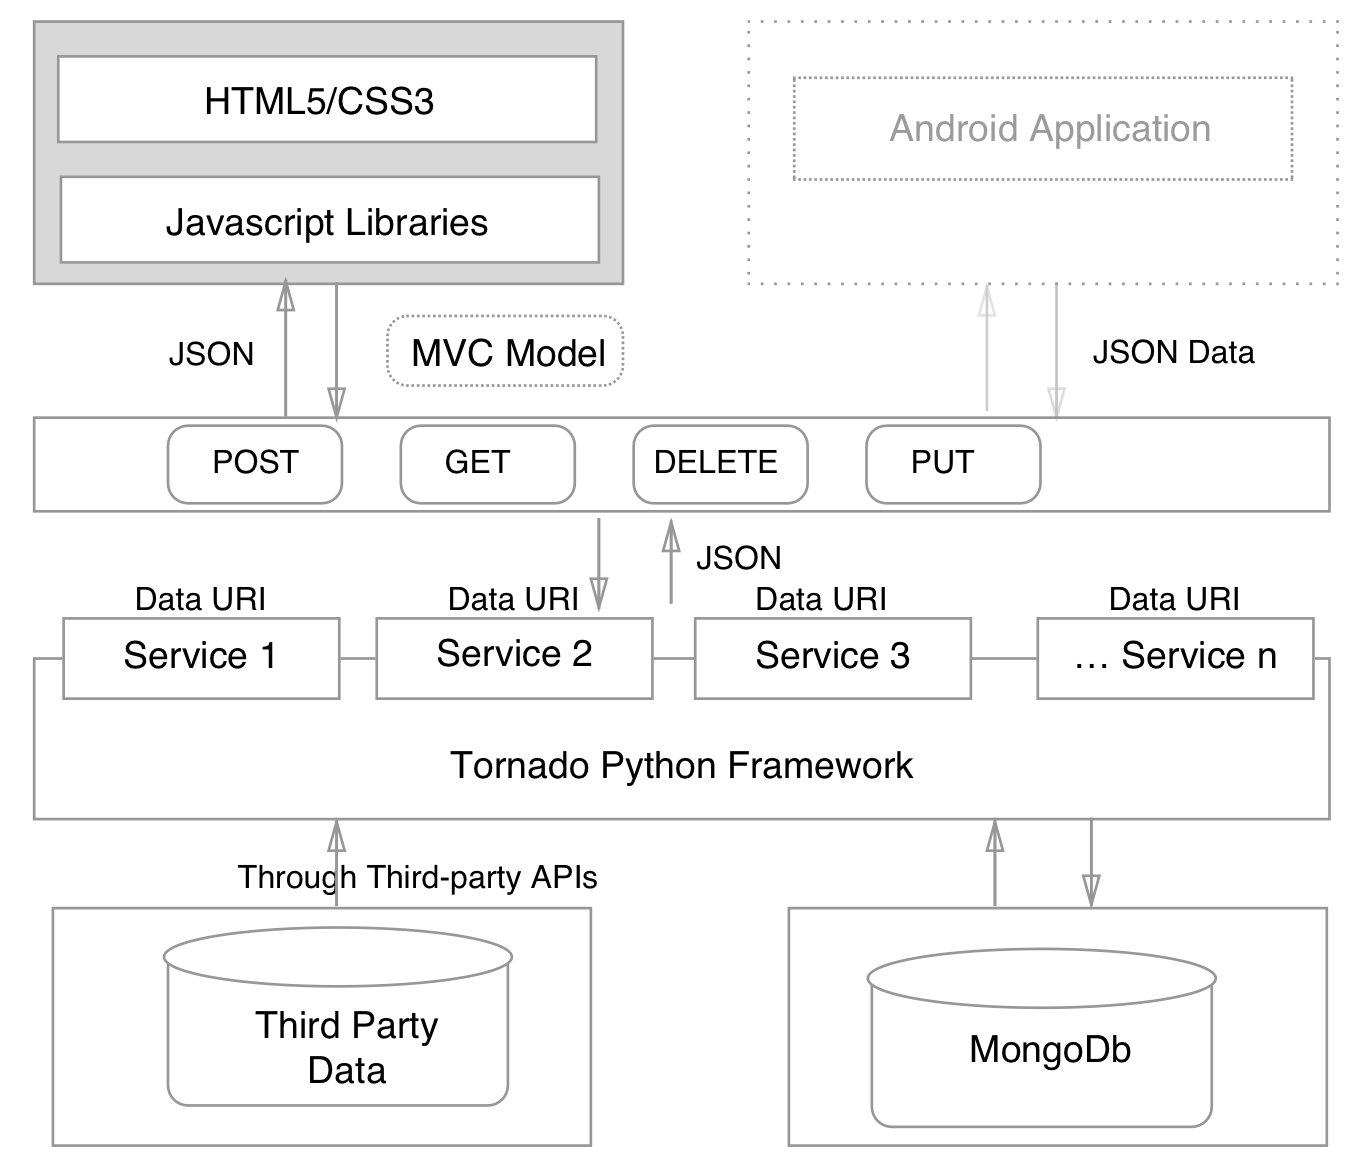
\includegraphics[width=12cm]{images/wegoo_web_building_blocks.png} % This scales the picture to
                                      % a width of 10cm
                                      % You can scale to the
                                      % width or height you need
%\end{center}
\caption{Server Application design diagram}
\label{fig:fig-eg}
\end{figure}


The figure above shows for every components the technology associated. The web application is build using python and takes the advantages of the python data processing capabilities. The basic aim of the web application is to provide the linkage between the experienced Doctors and nursers after further investigation on the data is carried out. The technologies illustrated in the above figure was chosen to make the data access and processing smooth and easy to ready including:
\begin{enumerate}
	\item The entire application is build on top of RESTful services. As Roy Fielding introduced REST (Representational state transfer) in his Doctoral dissertation, REST provides a component based style with a clear interconnection of the components as well as the data exchange between the components. The distributed comments of the system communicate but not always through HTTP (HyperText Transfer Protocol) and with the help of different REST and HTTP verbs like GET, POST, PUT and DELETE components can request through data URIs (Uniform Resource Identifies). for instance, GET /data/api/v/56779f77b38b4664dcf6d165 shows a data URI to get information of a particular patient when Patient ID number is provided\cite{fieldingarchitectural}
	\item {\bfseries Tornado}: is a python web framework that was developed original by FriendFeed. It is an asynchronous network library and it can handle many open connection due to its using non-blocking network I/O. Tornado was chosen in this work for it provides the capability of developing a distributed components based architecture, and it is suitable building data intense real time web applications dues to its supports of long pulling and web sockets. the following code snippets shoes an example of a simple Tornado application
\begin{figure}[H]
\centering
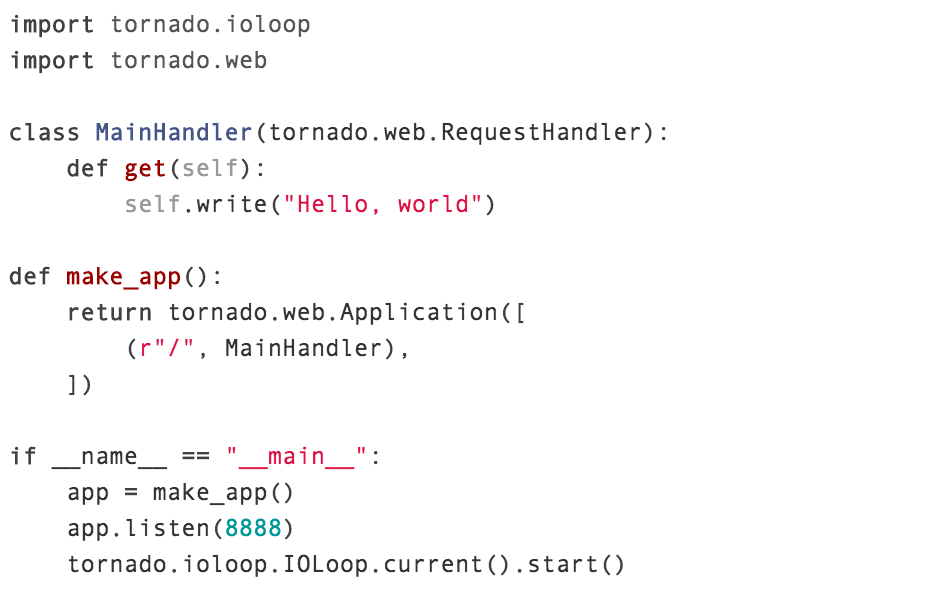
\includegraphics[width=11cm]{images/tornado_sample_app.png} % This scales the picture to
                                      % a width of 10cm
                                      % You can scale to the
                                      % width or height you need
%\end{center}
\caption{Tornado python framework application skeleton}
\label{fig:fig-eg}
\end{figure}
	\item {\bfseries mongoDB} module was used to store the data from the android mobile application and to update the website. The information are stored into collections and each patient entry is classified as a document in the patient information collection. MongoDB is an open source cross-platform non-SQL database, in other words it is a document-oriented databases since it avoids the familiar SQL based databased structure of the table based and relational based databases. mongoDB makes the integration of data into application more easily since it provides data into JSON-like formants in the form of documents. Its flexible schemas allows the integration to store different kind of information in one place with key-value format \cite{mongodb2016}.
\end{enumerate}
